\paragraph{Shared Q-tables and the placebo.} \citet{esquinas2026} find that the
price-trigger signature at $\xi=500$ is sharpest when both traders read and
update a single \emph{shared} Q-table, and that this protocol also yields
much higher collusion indices ($0.87$--$0.92$). A shared table is one learner
choosing for several traders, so we apply the same placebo to it.
Table~\ref{tab:shared} and Figure~\ref{fig:shared} show the results. Sharing
raises the index for forward-looking learners to $\SharedKyleStratDeltaInt$
($\xi=0$) and $\SharedDouStratDeltaInt$ ($\xi=500$), and for myopic learners to
$\SharedDouMyopicDeltaInt$ in both regimes, the level reported for shared tables
in the replication, reached by a learner that cannot collude.

The noise-shock test then fails the placebo. At $\xi=500$ the \emph{myopic}
shared learner ignores small shocks ($\SharedDouMyopicShockSmall\%$ of $\beta^N$
for a shock of $0.05$ deviation units) but trades harder after larger ones
($\SharedDouMyopicShockMid\pm\SharedDouMyopicShockMidCI\%$ at $0.25$ and
$\SharedDouMyopicShockLarge\pm\SharedDouMyopicShockLargeCI\%$ at one deviation
unit): the threshold pattern that \citet{dou2025} interpret as a price
trigger. A learner with $\gamma=0$ cannot be punishing anyone, so this response
cannot be a punishment strategy. The forward-looking shared learner shows no
significant response at our horizon. A natural explanation, which we check
in Appendix~\ref{app:rare}, is that large shocks push the market into
rarely visited price states, where estimates have been updated less often and
therefore pruned less, so the learned orders there are more aggressive. Under
pruning, the response of a Q-learner to a price shock depends on how often the
resulting state has been visited, so a threshold-like reaction can arise
without any strategy. The noise-shock test therefore needs the placebo to be
informative: a reaction identifies punishment only if a myopic learner trained
in the same way does not show it.

\begin{table}[t]
  \centering
  \small
  \resizebox{\linewidth}{!}{\begin{tabular}{llcccccc}
\toprule
$\xi$ & Shared Q-table & $\Delta$ intensity & \multicolumn{3}{c}{Shock response (\% of $\beta^N$)} & Rival reaction & Seeds \\
 & & & 0.05 & 0.25 & 1 & (\% of $\beta^N$) & \\
\midrule
0 & $\gamma=0.95$ & $0.68 \pm 0.00$ & $0.12 \pm 0.13$ & $0.15 \pm 0.35$ & $-0.06 \pm 0.68$ & $0.10 \pm 0.51$ & 1 \\
0 & $\gamma=0$ (myopic placebo) & $0.86 \pm 0.00$ & $-0.05 \pm 0.11$ & $0.04 \pm 0.22$ & $0.53 \pm 0.59$ & $0.07 \pm 0.45$ & 1 \\
500 & $\gamma=0.95$ & $0.62 \pm 0.00$ & $0.65 \pm 0.59$ & $0.27 \pm 0.74$ & $-0.33 \pm 0.75$ & $0.18 \pm 0.77$ & 1 \\
500 & $\gamma=0$ (myopic placebo) & $0.71 \pm 0.00$ & $0.25 \pm 0.14$ & $1.07 \pm 0.23$ & $4.04 \pm 0.33$ & $2.98 \pm 0.24$ & 1 \\
\bottomrule
\end{tabular}}
  \caption{Shared Q-tables in the \citet{dou2025} calibration
  ($1.5\times10^7$ periods, 100 markets). Shock response: change in per-trader
  intensity one period after a noise shock of the given size in deviation
  units, as a percentage of $\beta^N$. Rival reaction: change in rivals'
  intensity one period after a forced best-response deviation. 95\% CIs.}
  \label{tab:shared}
\end{table}

\begin{figure}[t]
  \centering
  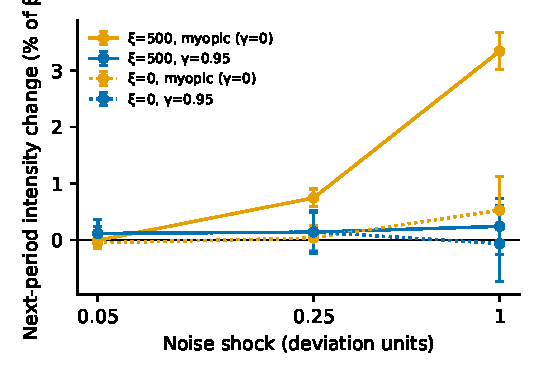
\includegraphics[width=0.5\linewidth]{figures/fig_shared.pdf}
  \caption{Noise-shock responses with shared Q-tables. At $\xi=500$ the myopic
  placebo (orange, solid) ignores small shocks and reacts to large ones, the
  threshold pattern read as a price trigger, although with $\gamma=0$ it has no
  reason to punish.}
  \label{fig:shared}
\end{figure}
